\chapter{NMR-EsPy walkthroughs}
The remainder of this thesis is an insert from the documentation of
version 2.0 of \acs{EsPy}. The section of the documentation included provides
walkthroughs describing how to use the package's \ac{API} for the consideration
of \ac{1D} and \ac{2DJ} \ac{NMR} datasets \note{Sequential data too?}. These
walkthroughs provide a short description of the key features associated with
the package, and is an ideal first place to get up-and-running with using it.

Also included in the full documentation are instructions on installation
and using the \acp{GUI} for \ac{1D} and \ac{2DJ} estimation, and a complete
reference for the complete \ac{API}. The most up-to-date version of the
documentation can be found at:
\begin{itemize}
    \item[] \textbf{HTML:} \url{https://foroozandehgroup.github.io/NMR-EsPy/}
    \item[] \textbf{PDF:} \note{???}
\end{itemize}
The source code for \ac{EsPy} is hosted on the Foroozandeh group's GitHub page
at \url{https://github.com/foroozandehgroup/NMR-EsPy}.

\includepdf[%
    pages={13-28},%
    addtotoc={1,subsection,1,Hello,p1},%
    pagecommand = {\thispagestyle{fancy}},%
    offset=0 -1cm,%
]{nmr-espy.pdf}
